\chapter{Vectors} \label{ch:vectors}

When visualising vectors as arrows, always think of them as being rooted in one spot.

When in physics we speak of a "vector field", that is, a vector at each point in space, such as wind speed and direction, or the electric field, we visualise arrows spread out over space. But the value of the field in two different places may be the same.

This is obvious (and less confusing) in the case of a scalar field, such as temperature. At two different locations in a room, the temperature may be the same. It's a numerical value that varies from place to place, and the same number may appear in two places.

But exactly the same is true for a vector field. If the wind is some particular speed and direction at two different places on the map, we say the vectors are equal: they are the \textit{same vector}. It is irrelevant that they are associated with different locations in physical space. In vector space, there is one vector with that direction and length.

\section{Vectors as geometric objects}\label{sec:vectors-geometric}

What is a two dimensional vector? A common starting point is to say it's two numbers, and we very often casually refer to a column like this as a vector:

$$
\begin{bmatrix}3 \\ 2\end{bmatrix}
$$

But one of the most important ideas in physics is that vectors are primarily geometric objects. They can be described with numeric coordinates, but there is no preferred coordinate basis. A vector has an independent existence.

To understand what we are giving up, it may help to initially visualise the space of plane vectors as having some intrinsic coordinate grid built into it, so every vector in that space "knows" its own numeric coordinates, being fixed to that grid.

\begin{figure}[h]
    \centering
    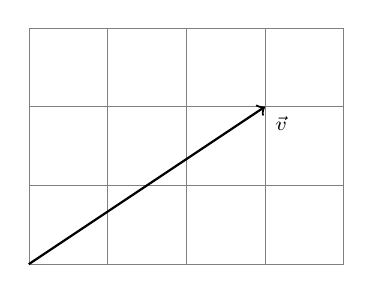
\begin{tikzpicture}
        \draw[step=1cm,gray,very thin] (0,0) grid (4,3);
        \draw[thick,->] (0,0) -- (3,2) node[anchor=north west] {\scriptsize $\vec{v}$};
    \end{tikzpicture}
    \caption{A vector on a fictional grid.} \label{fig:vector-grid}
\end{figure}

But in physics, our vectors relate to something in nature that has a magnitude and an an alignment, and there is no grid unless we invent one.

For some unknown vector space that we assert to be two dimensional, a pair of numbers only describes a vector if we have a basis $\begin{bmatrix}\vec{e}_1 & \vec{e}_2\end{bmatrix}$.

\begin{figure}[h]
    \centering
    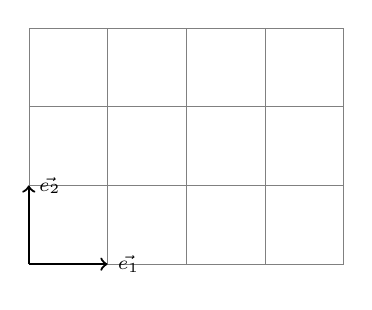
\begin{tikzpicture}
        \draw[step=1cm,gray,very thin] (0,0) grid (4,3);
        \draw[thick,->] (0,0) -- (1,0) node[anchor=west] {\scriptsize $\vec{e_1}$};
        \draw[thick,->] (0,0) -- (0,1) node[anchor=west] {\scriptsize $\vec{e_2}$};
    \end{tikzpicture}
    \caption{A basis that properly defines a grid.} \label{fig:vector-basis}
\end{figure}

Matrix multiplication (§\ref{sec:matrix-multiplication}) between a row of basis vectors and a column of scalars produces a sum of vector terms:

$$
\begin{bmatrix}\vec{e}_1 & \vec{e}_2\end{bmatrix}
\begin{bmatrix}3 \\ 2\end{bmatrix}
= 3\vec{e}_1 + 2\vec{e}_2
$$

A property of a vector is that you can multiply it by a scalar to get another vector (unless you multiply by 1, in which case you get the same vector), and another property is that you can add two vectors (placing them end to end) to get another vector. So an expression such as:

$$3\vec{e}_1 + 2\vec{e}_2$$

describes a new vector that we have produced by mixing together two basis vectors. 

\begin{figure}[h]
    \centering
    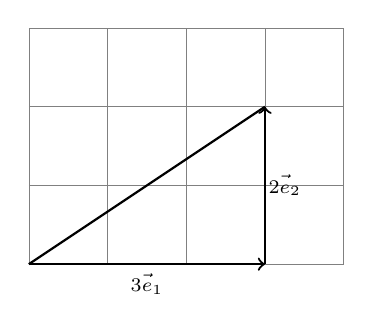
\begin{tikzpicture}
        \draw[step=1cm,gray,very thin] (0,0) grid (4,3);
        \draw[thick,->] (0,0) -- (3,0);
        \node at (1.5,-0.25) {\scriptsize $\vec{3e_1}$};
        \draw[thick,->] (3,0) -- (3,2);
        \node at (3.25,1) {\scriptsize $\vec{2e_2}$};
        \draw[thick] (0,0) -- (3,2);
    \end{tikzpicture}
    \caption{Sum of scaled basis vectors.} \label{fig:vector-sum}
\end{figure}

Any vector in the space can be described in this way. And therefore any vector can be decomposed into coordinates, but only once you have chosen some basis vectors.

It's not necessarily possible to say anything numerically about a single vector, because it can't be described numerically without introducing basis vectors to measure it against. A vector has a length and a direction, but these things can only be measured in relation to other vectors.

A vector space is a set of vectors, and we can if we like think of the vectors in the space as having an absolute existence, but we cannot say that there is one correct perspective to view those vectors from, any more than we can assume the North Pole is the "top" of the Earth, nor one correct scale to measure them by.

All we can say is that there is some angle between two vectors, or some ratio between the lengths of two vectors.

It follows that we cannot meaningfully communicate our choice of basis to anyone in terms of that basis alone. The coordinates of our two chosen basis vectors, if we express them in terms of our basis itself, are always:

\begin{equation}   
    \begin{split}
        e_1 &= \begin{bmatrix}1 & 0\end{bmatrix} \\
        e_2 &= \begin{bmatrix}0 & 1\end{bmatrix}
    \end{split}
\end{equation}

That is, $\vec{e}_1$ contains 1 unit of itself and nothing of $\vec{e}_2$, and the reverse situation for $\vec{e_2}$. This is like saying "it is what it is." It looks like the identity matrix (this is not a coincidence):

$$
\begin{bmatrix}1 & 0 \\ 0 & 1\end{bmatrix}
$$

The realisation of this relativistic nature of vectors can produce confusion, just as may occur when we first encounter the idea that position in physical space is not absolute, velocity is not absolute, etc. It just has to be accepted. But we can suppose the existence of an intrinsic hidden absolute basis, a coordinate grid, and use this as a mental crutch to stabilise ourselves, while gradually developing an understanding that this crutch is not necessary.

The question remains: how do we identify a set of basis vectors? If we have an inner product then we can pick an orthonormal basis, because we can make sure each basis vector is of unit length (inner product with self is $1$) and all are mutually orthogonal (inner product is $0$).

\section{Vector Spaces}\label{sec:vectors-space}

If vectors are not merely collections of numbers it's important to be clear what they are. A vector space is a set of objects that meet certain abstract criteria. As soon as we can identify a way of meeting all the criteria, the set of objects is a vector space and the objects are vectors.

It may be worth throwing out any preconceptions about vectors based on picturing arrows drawn on grid paper and just say that there is a set of mysterious "objects" of which we will state some abstract properties, but leave anything else unspecified.

\subsection{They can be added}

There is an operator $+$ that takes two objects from the set and returns another from the same set (so it's a closed operator).

This operator is commutative:

$$\vec{u} + \vec{v} = \vec{v} + \vec{u}$$

and associative:

$$\vec{u} + (\vec{v} + \vec{w}) = (\vec{v} + \vec{u}) + \vec{w}$$

There is a special object called $0$, which makes no difference when added to any object from the set:

$$\vec{v} + 0 = \vec{v}$$

Also every object has an opposite, known as its additive inverse, so they pair up. The inverse of $\vec{v}$ is written as $-\vec{v}$, and:

$$\vec{v} + (-\vec{v}) = 0$$

The above can written as $\vec{v} - \vec{v}$.

\subsection{They can be scaled}

There is an associated set of objects called scalars, typically restricted to real or complex numbers. Our objects can be multiplied by a scalar to get another object. Scaling them by $1$ makes no difference. Scaling them by $-1$ discovers the additive inverse.

Given two scalars $a$ and $b$, we can compute $c = ab$ and then scale an object $\vec{v}$ by it, or we can separate scale the object first by $a$ and then by $b$, and the result is the same:

$$(ab)\vec{v} = a(b\vec{v})$$

Scaling is distributive over addition of objects:

$$a(\vec{u} + \vec{v}) = a\vec{u} + a\vec{v}$$

And also over addition of scalars:

$$(a + b)\vec{v} = a\vec{v} + b\vec{v}$$

\subsection{The Field}

A vector space's set of scalars is known as its field. It can be any sort of object for which we can define addition, subtraction, multiplication and division, so real or complex numbers usually serve this purpose, but there exist vectors that cannot serve as a field of scalars for other vector spaces. For example, familiar geometric vectors cannot be multiplied and divided in a way that is closed.

\subsection{Examples of Vector Spaces}

Any set of objects for which we can define these operations is a vector space. This means that the real numbers $\mathbb{R}$ and complex numbers $\mathbb{C}$ themselves qualify as vector spaces, although with the proviso that you have to choose the field appropriately. You can't have a vector space of $\mathbb{R}$ over the field of $\mathbb{C}$, because the product of a vector from $\mathbb{R}$ and a scalar from $\mathbb{C}$ is very often going to be a member of $\mathbb{C}$ but not of $\mathbb{R}$, that is, not a vector.

Ordered pairs of real numbers, $\mathbb{R}^2$, clearly also qualify, because addition can add the first and second pair members separately, scaling can scale both of the members, and then all the other requirements follow automatically.

The example of $\mathbb{C}$ as a vector space is particularly interesting because it is essentially identical to $\mathbb{R}^2$. The only difference is that it defines multiplication as a closed operation over its vectors (such that the product of two vectors is a vector), which is absolutely not a general feature of vector spaces.\footnote{Although it is also defined (very differently) in $\mathbb{R}^2$ as the cross product, $\times$.}

\section{Dot Product}

Also known as the scalar product (an exact synonym), sometimes as "the inner product" (not an exact synonym, as we'll see).

The dot product is a scalar-valued operator between two vectors, $\vec{p}\cdot\vec{q}$. It has the same scalar value under a change of coordinate system, as long as the basis vectors remain the same length and orthogonal (i.e. under rotation or reflection).

If the two vectors $\vec{p}$ and $\vec{q}$ are separated by angle $\theta$, and we know the magnitude (length) of each vector, e.g. $\|\vec{p}\|$, then

$$
\vec{p}\cdot\vec{q} =
\|\vec{p}\| \|\vec{q}\|\cos{\theta}
$$

Aside from the immediately obvious fact that it is commutative (swapping the vectors makes no difference), the behaviour of $\cos$ has some implications.

First, as $\cos{0} = 1$, for vectors pointing in the same direction we just multiply their magnitudes. Further, the dot product of a vector with itself is the square of the magnitude:

$$\vec{p}\cdot\vec{p} = \|\vec{p}\|^2$$

And of course if it's a unit vector, the result is $1^2 = 1$.

Second, as $\cos{\pi} = -1$, for vectors pointing in opposite directions, the result is the same but negative: $-\|\vec{p}\| \|\vec{q}\|$.

Third, as $\cos(\pi/2) = \cos(3\pi/2) = 0$ orthogonal vectors have dot product equal to zero. So given a Euclidean basis (a set of orthonormal basis vectors) $\vec{e_n}$:

$$\vec{e_i} \cdot \vec{e_j} = \delta_{ij} $$

Note that this is an observation about a set of orthonormal vectors, so even though we've used indices to label directions, we aren't talking about coordinates \textit{yet}.

\subsection{Finding coordinates}

It's also interesting to consider the dot product of any vector $\vec{p}$ with a unit vector, such might make a suitable basis vector $\vec{e_n}$. If $\vec{p}$ is in the same direction as $\vec{e_n}$, the dot product is just $\|\vec{p}\|$. If orthogonal, it's zero.

For angles between, consider the right triangle, where:

$$\cos \theta = \frac{adjacent}{hypotenuse}$$

So if the hypotenuse is our vector $\vec{p}$, hence of length $\|\vec{p}\|$ and the side adjacent to $\theta$ is a vector in the same direction as one of our unit basis vectors $\vec{e_n}$ scaled by some factor we will call $p_n$, which is therefore the magnitude of that vector and the length of the adjacent side:

$$\cos \theta = \frac{p_n}{\|\vec{p}\|}$$

Then:

$$
\vec{p}\cdot\vec{e_n}
= \|\vec{p}\| \|\vec{e_n}\|\cos{\theta}
= \|\vec{p}\| \|\vec{e_n}\|\frac{p_n}{\|\vec{p}\|}
= \|\vec{e_n}\|p_n
$$

But $\vec{e_n}$ is a unit vector so $\|\vec{e_n}\|$ is 1, and therefore:

$$
\vec{p}\cdot\vec{e_n} = p_n
$$

So it is the \textit{projection} of $\vec{p}$ on to $\vec{e_n}$, which is to say it is the $n$-th coordinate, $p_n$ of $\vec{p}$. Thus we can reconstitute $\vec{p}$ by summation:

$$
\vec{p}
= \sum_n{\vec{e_n} p_n}
= \sum_n{\vec{e_n} \left( \vec{p} \cdot \vec{e_n} \right)}
$$

That is, $\vec{p}$ is the sum of its component vectors, each of which is a basis vector scaled by a coordinate, that coordinate being the result of the dot product between $\vec{p}$ and the basis vector.

\subsection{Dot Product is Homogeneous}

Intuitively, a triangle scales linearly. If the hypotenuse is scaled by some factor $k$, the adjacent side will also scale by $k$:

$$
k(\vec{p}\cdot\vec{e_n})
= (k\vec{p})\cdot\vec{e_n}
$$

So the dot product is \textit{homogeneous}.

\subsection{Dot Product is Distributive}

Vector addition also has a useful simplifying property. Consider two vectors $\vec{q}$ and $\vec{r}$. Each has a component along basis vector $\vec{e_n}$, so:

$$\vec{q} \cdot \vec{e_n} = q_n$$
$$\vec{r} \cdot \vec{e_n} = r_n$$

If we picture $\vec{q}$ and $\vec{r}$ laid head to tail, the total distance travelled in the direction of $\vec{e_n}$ is $q_n + r_n$, or:

$$
\vec{p} \cdot (\vec{q} +\vec{r} )
= \vec{p} \cdot \vec{q} +\vec{p} \cdot \vec{r}
$$

This means the dot product is \textit{distributive} over vector addition.

\subsection{Do not interchange scalar and dot product}

It may be worth drawing attention to a tempting manipulation that is not valid:

$$
\vec{p} \left( \vec{q} \cdot \vec{r} \right) \ne \vec{q} \left( \vec{p} \cdot \vec{r} \right)
$$

Each side multiplies either $\vec{p}$ or $\vec{q}$ by a scalar. It doesn't matter that the scalar is obtained from the dot product; it's just a scalar. Multiplying a vector by a scalar will not change its direction, so there is no reason the results will be in the same direction.

\section{Using coordinates}

Having done the hard work (computing $\cos$) in order to obtain the coordinates, things subsequently become much easier. Given a basis $\vec{e_n}$ and a pair of vectors, $\vec{p}$ and $\vec{q}$, with coordinates $p_n$ and $q_n$, so:

$$\vec{p} = \sum_n \vec{e_n}p_n$$
$$\vec{q} = \sum_n \vec{e_n}q_n$$

For the dot product, using the coordinate form of $\vec{p}$:

$$
\vec{p}\cdot\vec{q} =
\left[ \sum_n{\vec{e_n}p_n} \right] \cdot \vec{q}
$$

As the dot product is distributive over addition, that means we can move it inside the summation:

$$
\vec{p}\cdot\vec{q} =
\sum_n \left[ \vec{e_n} p_n \cdot \vec{q} \right]
$$

And because it is homogeneous, we can gather the vectors:

$$
\vec{p}\cdot\vec{q} =
\sum_n p_n \left[ \vec{q} \cdot \vec{e_n} \right]
$$

But $\vec{q} \cdot \vec{e_n}$ is the projection of $\vec{q}$ on to $\vec{e_n}$, that is, it is the coordinate $q_n$ of $\vec{q}$ in the direction of $\vec{e_n}$, so:

$$
\vec{p}\cdot\vec{q} = \sum_n p_nq_n
$$

And so for two vectors expressed as coordinates in a common basis, we just multiply their corresponding coordinates and sum the results, which is ridiculously simple (no $\cos$ at all), and which is why the coordinate approach is so attractive for calculation.

In the case where $\vec{p} = \vec{q}$:

$$
\vec{p}\cdot\vec{p} = \sum_j {p_j}^2
$$

Which is Pythagorus's theorem, agreeing with our earlier claim that the dot product of a vector with itself is the square of the magnitude.

\section{Change of Basis}\label{sec:vectors-change-basis}

A matrix can be used to:

\begin{itemize}
    \item map vectors to a new length and direction in the same basis, or
    \item perform a coordinate conversion on vectors so they remain the same vectors but expressed in different numerical coordinates.
\end{itemize}

The mathematical machinery is identical.

Viewed as an operator, the matrix may have eigenvectors only in some directions. The operator is therefore a geometrical object just as a vector is, and the matrix elements may be numerically different depending on the basis, just as the coordinates of a vector may differ depending on the basis, despite describing the very same objects regardless of the basis chosen.

Viewed as a coordinate converter, the matrix effectively depends on two bases, the one being converted from and the one being converted to.

\subsection{Effect of change of basis on vectors}

A plane vector $\vec{v}$ in some basis can be expressed in coordinates as a column matrix $V$:

$$V = \begin{bmatrix}3 \\ 4\end{bmatrix}$$

And with the basis as a row matrix:

$$E = \begin{bmatrix}\vec{e_1} & \vec{e_2}\end{bmatrix}$$

Matrix multiplication builds the vector:

$$\vec{v} = EV = 3\vec{e_1} + 4\vec{e_2}$$

We can create a matrix that will double the length of the basis vectors:

$$G = \begin{bmatrix}2 & 0 \\ 0 & 2\end{bmatrix}$$

By the rules of matrix multiplication the bases needs to be on the left:

$$E' = EG = \begin{bmatrix}2\vec{e_1} & 2\vec{e_2}\end{bmatrix}$$

What coordinates would $\vec{v}$ have in this new basis $E'$? Intuitively the coordinates need to be halved to refer to the same vector. So we need the inverse of $G$, written as $G^{-1}$, which shrinks the coordinates, so we'll call it:

$$S = G^{-1} = \begin{bmatrix}0.5 & 0 \\ 0 & 0.5\end{bmatrix}$$

And so our vector's coordinates become:

$$V' = SV = \begin{bmatrix}1.5 \\ 2\end{bmatrix}$$

This is the same vector as before, just in different coordinates:

$$\vec{v} = EV = E'V'$$

We say that vectors are \textit{contravariant} under a change of basis.

\subsection{Dot product under change of basis}

The dot product depends on the lengths of two vectors and the angle between them. If the vectors are represented as coordinates in some basis, then a change of basis will change the coordinates. Will the dot product change too? It depends.

If the basis vectors are only rotated (all by the same angle) or reflected, this preserves both lengths and angles, so the dot product will be unaffected. Operators that preserve the dot product are known as \textit{unitary}.

If the basis vectors are scaled, the lengths implied by the coordinates will change and so the dot product will change. To take the above example, we grow the basis vectors with $G$, having the equivalent effect on the coordinates to shrinking the input vectors with $S$ to half their original length, and so the dot product will be $\frac{1}{4}$ of its original value.

If the basis vectors are skewed, this will have the equivalent effect on the coordinates of skewing the input vectors, changing the angle between them.

\section{Covectors}

A covector is a scalar-valued linear function of a vector that performs the dot product using a pre-determined other vector.

$$f_n(\vec{v}) = \vec{e_n} \cdot \vec{v}$$

In other words, every vector has a corresponding covector which extracts a coordinate along the direction of that vector.

It can be expressed as a row matrix with scalar components. For example the coordinates of a basis vector $\vec{e_n}$ could be written as a row matrix:

$$E_n = \begin{bmatrix}1 & 0\end{bmatrix}$$

This is a covector, distinguished by being a row rather than a column. So to apply the covector is just matrix multiplication:

$$E_nV$$

where $V$ is the column matrix of the coordinates of the input vector $\vec{v}$.

We can construct such a function for all $n$ basis vectors, and these form a basis in the so-called dual space of all possible covectors, which is itself a vector space, each covector being defined by only by a set coordinates.

Following the above narrative our $\vec{v}$ is now expressed as $V'$, having been shrunk by $S$ to work in basis $E'$. We now want evaluate $F_n$ on $V'$, but there is an incompatibility of basis, because $F_n$ has the $n$-th basis vector of $E$ in its definition.

Or to put it simply, the coordinates in $V'$ have been shrunk, whereas $F_n$ only works correctly with unshrunk coordinates.

We can fix this by pre-converting the input vector:

$$E_nGV$$

This new covector applies matrix $G$ to the input, growing it so it becomes compatible with $E_n$. But as can be easily verified, it makes no difference to the result whether we evaluate $GV$ or $E_nG$ first; this is the beauty of linear functions. Thus we can produce an amended row-matrix based on the original:

$$E'_n = E_nG$$

It has a built-in "growth factor", and so is compatible with vectors that have been shrunk.

This means that under a change of coordinate systems, where the basis vectors have had $G$ applied to them, covectors must also have $G$ applied to them. This is the opposite of what has to happen to vectors.

As a result we say covectors are \textit{covariant} (this is the source of the name covector).

\section{Operators}

An operator $\hat{O}$ is a function that maps from vectors to vectors. That is, the input is a vector and so is the output. It may change the length or direction of the vector.

We are particularly interested in linear operators, for which:

$$\hat{O}(x\vec{i} + y\vec{j}) = x\hat{O}\vec{i} + y\hat{O}\vec{j}$$

Why? Because if you have chosen your basis $\vec{i}, \vec{j}$ and so you can express all vectors in coordinates $(x, y)$, i.e. as simple "weighted sums" of your two basis vectors, $x\vec{i} + y\vec{j}$, then to apply $\hat{O}$ to a vector, all you need to know is $\hat{O}\vec{i}$ and $\hat{O}\vec{j}$.

By applying the operator to the basis vectors, you discover two new basis vectors:

$$\vec{i'} = \hat{O}\vec{i}$$
$$\vec{j'} = \hat{O}\vec{j}$$

The coordinates you would use to express an input vector:

$$\vec{v} = x\vec{i} + y\vec{j}$$

can be used to mix these new basis vectors and get the result of applying the operator to the input vector:

$$\hat{O}\vec{v} = \hat{O}(x\vec{i} + y\vec{j}) = x\vec{i'} + y\vec{j'}$$

A matrix can be interpreted as a way to convert coordinate vectors from one basis to another, preserving the same meaning, or as a way to produce a different vector in the same basis.

Considering the latter use, i.e. linear operators that transform vectors, what effect does a change of basis have on vector coordinates?

\section{Eigenvectors and Eigenvalues}\label{sec:vectors-eigen}

An operator that performs only scaling (e.g. $G$ and $S$) is isotropic, treating all directions equivalently.

But some operators are biased with regard to direction. To characterise the behaviour of an operator we can consider those vectors which are scaled by it without their direction being altered (the scaling may be negative, leaving the vector pointing the opposite direction; as long as the resulting vector is co-linear with the input vector, that's insignificant enough.) Such vectors are called the \textit{eigenvectors} of the operator, and the corresponding scalar values are the \textit{eigenvalues}.

So in the case of $S$ and $G$, all input vectors are eigenvectors: all inputs get only scaled, and always by the same eigenvalue.

With vectors in the plane, when the operator is a pure rotation, e.g. by a right-angle anti-clockwise:

$$R_A = \begin{bmatrix}0 & -1 \\ 1 & 0\end{bmatrix}$$

or clockwise:

$$R_C = \begin{bmatrix}0 & 1 \\ -1 & 0\end{bmatrix}$$

every vector changes direction by the same angle, and that means there are no eigenvectors.

The zero vector is not considered a candidate for an eigenvector; regardless of the operator, it goes from length zero to length zero, so any scalar could be the eigenvalue, meaning that the eigenvalue is undefined.

In three dimensions the rotation has an axis, along which all vectors are eigenvectors. Curiously, even though these vectors don't exist in the plane, we can find \textit{complex} eigenvalues for them by supposing that such eigenvectors exist, which is weird.

More interestingly, there are operators for which only some vectors are eigenvectors. Consider a reflection (call it $M$ for mirror):

$$M = \begin{bmatrix}1 & 0 \\ 0 & -1\end{bmatrix}$$

If we take the first coordinate to be horizontal and the second vertical, this flips the input vector to point up rather than down, or vice versa. So it seems that all vectors have their direction changed and are not eigenvectors, but there exceptions: vectors that lie on the horizontal axis and have no vertical component will be unaffected, i.e. they will be eigenvectors with eigenvalue 1. Also vectors that lie on the vertical axis will have their direction changed, but to the exact opposite direction (their alignment does not change), which is the same as being scaled by -1, and so these too are eigenvectors, but with eigenvalue -1.

So within the space of input vectors, there is a subspace (the \textit{eigenspace}) of eigenvectors, and $M$ has an intrinsic orientation, as there is a particular line around which reflection occurs.

We can find the eigenvectors given a matrix representation $M$ of an operator acting on a vector represented by a column matrix $v$. If $v$ is an eigenvector, and $x$ is the corresponding eigenvalue, what we mean by that is:

$$Mv = xv$$

For the vector $v$, multiplying it by the matrix $M$ is the same as multiplying it by the ordinary number $x$. So with trivial algebra:

$$Mv - xv = 0$$

This is fine because $Mv$ and $xv$ are column matrices, and here $0$ is the column matrix filled with zeros.

Pulling out $v$ as a factor (not quite as trivial):

$$(M - xI)v = 0$$

We have to leave behind the identity matrix $I$ in place of $v$ because we need the matrix equivalent of the ordinary number $x$, so we can subtract it from $M$.

Having split it into two factors whose product is zero, we know that either one or both of the factors must be zero. We already realised we aren't interested in the case where $v$ is the zero vector because its eigenvalue will be undefined (it could be anything). So we refuse to accept $0$ as an eigenvector. Therefore $v$ is not the zero vector, and so the matrix $M - xI$ must be such that it is able to transform some non-zero vector $v$ into the zero vector. This means it has no inverse, as there is no way to recover the direction of the original vector if we've sent it to $0$ (the zero vector has no direction, or has all directions, so direction is a meaningless concept for it.)

One way to picture the effect of a matrix is to think of it acting on a unit square (where the matrix is $2 \times 2$) and asking what the area of the resulting parallelogram will be. If it is not zero, every point in the original square has a unique point in the parallelogram and vice versa: the matrix is invertible. If the area is zero, the points of the original square have been crammed onto a line of $1$ dimension, so we have destroyed the information about where they came from in $2$ dimensions. All input vectors end up pointing in the same direction, and are only distinguished by length. No linear transform will be able to spread them back out into the correct different directions: the matrix is not invertible.

The area of that parallelogram (or in higher dimensions, the volume of an n-parallelepiped) is called the determinant of the matrix, $\det M$. If it's zero, the matrix is not invertible. And therefore, if:

$$\det{(M - xI)} = 0$$

then we definitely have some eigenvalues. The determinant can be expanded out into a polynomial expression in $x$ (there are various methods; a popular one is to get a computer to do it) and then solved by factoring to find all the $x$ values that make one of the factors $0$. We can then plug those $x$ values back into:

$$(M - xI)v = 0$$

one at a time, and solve to find the corresponding $v$. Thankfully all this can be mechanised.

\section{Symmetric Matrices}\label{ch:vectors-symmetric}

One interesting kind of operator is any represented by a symmetric matrix in some basis, so $M^\intercal = M$, or $M_{ij} = M_{ji}$ for all combinations of $i$ and $j$. So the diagonal elements are unconstrained, but all others have to match their diagonally-opposite element.

The curious thing about them is that their eigenvectors are orthogonal and completely span the vector space. That is, in an N dimensional space, they perform a scaling in all N available orthogonal directions, stretching or squishing.

This means that if you find the eigenvectors of the operator, you've found an orthogonal basis. This is hugely important in Quantum Mechanics (§\ref{ch:qm}), albeit with some modifications for complex numbers.

\section{Effect of Change of Basis on Operator}

If we apply $R_A$ to our two basis vectors, all our non-zero vectors' coordinates will need to change (while still being the same vectors, of course, just expressed in a new basis.) This means, just as we had to fix our covector, we now need to come up with the matrix $M'$ that mirrors around the same line as $M$ did in the un-rotated basis. We say that $M'$ and $M$ represent the same operator in different coordinate systems.

This time it will be a three step process:

\begin{itemize}
    \item adjust the input vector so it is expressed in $M$-compatible ("pre-rotation") coordinates
    \item apply $M$ to the pre-rotation coordinates, to get the reflected vector in pre-rotation coordinates
    \item adjust the reflected vector into post-rotation coordinates
\end{itemize}

As we applied $R_A$ to the basis vectors, that means we must have applied $R_C$ to all the column matrices representing our vectors in coordinate form (clockwise rotation being the inverse of anti-clockwise rotation). So the three steps appear to the left of our input $V$:

$$M'V = R_CMR_AV$$

In English, reading from the right, take the input $V$, rotate it anti-clockwise (to undo the clockwise rotation we assume has been performed on it), then apply the original $M$ matrix for reflection, then rotate clockwise.

As with the covector example, we can ditch the example input $V$ and just compute the matrix by itself for later use with any $V$:

$$M' = R_CMR_A$$

So the matrix $M'$ represents the same operator as $M$ in the anti-clockwise rotated coordinate system.

When it comes to classifying this as covariant or contravariant, we have a puzzle. It was necessary to perform both kinds of coordinate transformation here.

There is a general pattern to these examples, vectors, covectors and operators, which is captured in the notion of a tensor.

\section{Inner Product}

An inner product is a scalar-valued operator between two vectors:

$$\langle \vec{p},\vec{q}\rangle$$

A vector space equipped with such an operator is called an \textit{inner product space}. The most well known example is the dot product. To qualify as an inner product an operator must satisfy certain properties. It must be commutative:

$$\langle \vec{p},\vec{q}\rangle = \langle \vec{q},\vec{p}\rangle$$

This is obviously true for the dot product as we simply multiply matched components and then sum them. Denoting the $i$-th component by $p_i$ and $q_i$:

$$\sum_i p_i q_i = \sum_i q_i p_i$$

We also require:

$$\langle \vec{p}+\vec{r},\vec{q}\rangle = \langle \vec{p},\vec{q}\rangle + \langle \vec{r},\vec{q}\rangle$$

Again this is obviously true as it's just multiplying out each term of the summation:

$$\sum_i (p_i + r_i)q_i = \sum_i p_iq_i + r_iq_i$$

The inner product notation is simply telling what is true of each term.

The next requirement ($\alpha$ being some scalar constant) is therefore no surprise:

$$\langle \alpha \vec{p},\vec{q}\rangle = \langle \vec{p},\alpha \vec{q}\rangle = \alpha \langle \vec{p},\vec{q}\rangle$$

and so we are always just summing the product $\alpha p_i q_i$ and the order makes no difference to the result.

There are further requirements that are discarded in some contexts:

$$\langle \vec{p},\vec{p}\rangle \geq 0$$

For the Euclidean dot product we're squaring the coordinates $p_i$ so the result must be positive. But in Relativity (§\ref{ch:relativity}) we allow negative ("spacelike") intervals, which is why this requirement is not always applied.

Finally, $\langle \vec{p},\vec{p}\rangle = 0$ if and only if $\vec{p}$ is the zero vector. Again this could be untrue in Relativity if the time and space contributions cancel out ("lightlike").

Generalising on the dot product, we can introduce a second summation index $j$ and make all the combinations $p_iq^j$, and then decide how much of a contribution to the sum each combination should make by controlling it with a matrix $A^i_j$ and now per Einstein we can say:

$$p_i A^i_j q^j$$

Which is equivalent to putting the transpose of $\vec{p}$ on the left, the matrix $\mathbf{A}$ in the middle and $\vec{q}$ on the right and doing matrix multiplication (and it doesn't matter how we group the operations):

$$\vec{p}^\intercal\mathbf{A}\vec{q}$$

Indeed, the above requirements on an inner product effectively mean that any inner product must be expressible in this form.

In the standard dot product, we are only interested in the diagonal combinations, $p_i q_j$ where $i=j$, but this is equivalent to saying that $\mathbf{A}$ is the identity matrix $\delta$.

This idea is generalised further when considering complex vector spaces.

\section{Complex vector spaces}\label{ch:vectors-complex}

Any vector space is defined over a \textit{field}. This is unrelated to the physics meaning of "field", a value defined at each point in a space. Here a field is any set of objects with binary operators for addition, subtraction, multiplication and division that behave like those of the real numbers, so $\mathbb{R}$ is a field.

But as complex numbers meet this criterion therefore $\mathbb{C}$ is also a field, and therefore a vector space may be complex, and have complex coordinates.

Even the simplest non-trivial example, $\mathbb{C}^2$, is not directly imaginable, because although each vector requires two coordinates, each of those is a complex number incorporating a real and imaginary part, so each vector requires four real numbers to describe it, and so $\mathbb{C}^2$ can be mapped to $\mathbb{R}^4$, which is impossible to visualise directly.

Even so, concepts applicable to real vector spaces also work for complex, although with some modifications. The main issue is determining the modulus, for which we must introduce an inner product.

If we use the usual dot product definition then we have a problem because we naturally expect the modulus to be a positive real number. Summing the squares of the components of a complex vector could well produce a negative result, and then we need to take the square root to get the modulus, so the modulus wouldn't even be a real number.

To ensure $\langle \vec{u}, \vec{v} \rangle$ is real and positive, we amend the inner product so that we first take the complex conjugate of one its arguments:

$$
\langle \vec{u}, \vec{v} \rangle
=
\vec{u}^* \cdot \vec{v}
$$

This has the complicating side-effect that commutativity:

$$
\langle \vec{u}, \vec{v} \rangle
=
\langle \vec{v}, \vec{u} \rangle
$$

no longer applies. But who says it needs to? We instead make the requirement be:

$$
\langle \vec{u}, \vec{v} \rangle
=
\left[ \langle \vec{v}, \vec{u} \rangle \right]^*
$$

This is sometimes called conjugate symmetry. If all the components are real then complex conjugation makes no difference and commutativity is restored, so the nice thing is that we've amended the rule in a way that is "backward compatible" with real vectors.

This does mean that when taking the inner product of two different complex vectors, it matters which one we take the complex conjugate of. In physics the convention is to take the conjugate of the LHS vector.

The general form of the inner product, where we supply a matrix to control how to pair up and weight the coordinates, is similarly amended.

We use the dagger $^\dagger$ symbol to mean conjugate transpose, where we transpose a matrix (so turn a column vector into a row) and also take the complex conjugate of every element. It's equivalent to applying both $^\intercal$ and $^*$.

$$
\langle \vec{u}, \vec{v} \rangle
=
u^\dagger \mathbf{M} v
$$

As usual if $\mathbf{M}$ is $\delta$ then this reduces to the first definition given above. It should at least be be self-adjoint or Hermitian, which is to say that:

$$\mathbf{M}^\dagger = \mathbf{M}$$

That is, every element is the complex conjugate of its diagonally opposing element, and that therefore elements on the diagonal are real (they aren't moved by the transposition and so must equal their own complex conjugates).

A matrix like this is the complex equivalent of the real symmetric matrix for which we gave a definition (§\ref{ch:vectors-symmetric}).

Several other important facts about Hermitian operators can be derived: their eigenvalues are all real, their eigenvectors are orthogonal and span the space and so can be used to construct an orthonormal basis.

Another interesting kind of operator in complex spaces is those where:

$$\mathbf{U}^\dagger \mathbf{U} = I$$

i.e. the identity operator. These are known as unitary operators. They have the property of preserving the inner product (which is the same property we observed before for rotations and mirrorings):

$$\langle \vec{u}, \vec{v} \rangle = \langle \mathbf{U} \vec{u}, \mathbf{U} \vec{v} \rangle$$

If you have a Hermitian operator expressed by the matrix $M$ you can convert it to another representation by wrapping it in a transformation $T$ and its inverse:

$$M' = T M T^{-1}$$

If $T$ is unitary then $M'$ will be Hermitian, recognisable by the relationship between diagonally opposite matrix elements.